% This is auto-generated file: do not edit!
% Exported from microMathematics Plus, version 2.16


This example demonstrates how to
prepare and adjust a graphical
representation of a function. For
example, we want to plot three
different functions:
\begin{center}\begin{tabular}{c}
  $f(x) := 25 + 10 \cdot sin \left( \sqrt{ \left| x \right| } \right) $
\end{tabular}\end{center}
\begin{center}\begin{tabular}{c}
  $g(x) := \frac{2}{{e}^{ \left| x \right|  / 15}} \cdot f \left( x \cdot 50\right) $
\end{tabular}\end{center}
\begin{center}\begin{tabular}{c}
  $h(x) := min \left( f \left( x\right) ,\, g \left( x\right) \right) $
\end{tabular}\end{center}

The function argument that represents
the x-values will be taken for N
points within the interval [x1, x2]:
\begin{center}\begin{tabular}{ccc}
  $N := 300$ &
  $x1 := -30$ &
  $x2 := 30$ \cr
\end{tabular}\end{center}
\begin{center}\begin{tabular}{c}
  $x := \left[ x1,\, x1 + \left( x2 - x1 \right) / N \,..\, x2 \right]$
\end{tabular}\end{center}

After the functions and their arguments
are defined, you can add the plot box
using the ''New element'' button in the
action bar or ''Add function plot''
button from the tool bar:
\begin{center}\begin{tabular}{c} 
\includegraphics[resolution=320]{graphics/function_plot_fig1.png} \end{tabular}\end{center}
\begin{center}\begin{tabular}{c} 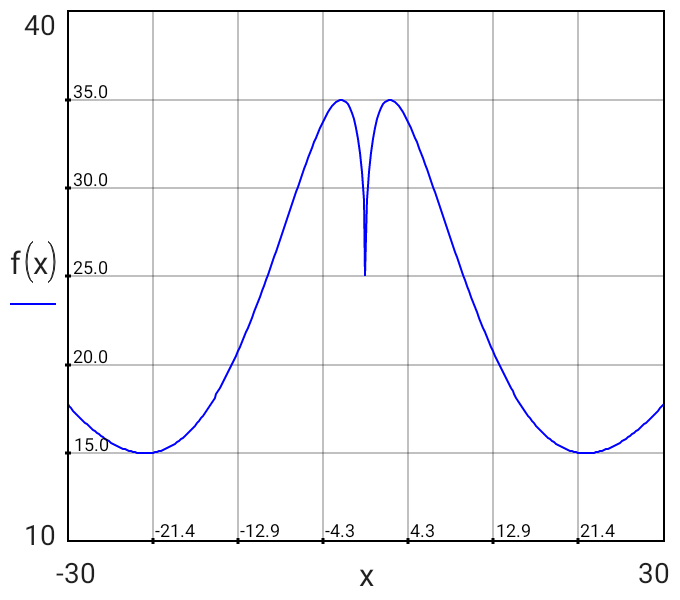
\includegraphics[resolution=320]{graphics/function_plot_fig2.png} \end{tabular}\end{center}

The function to be plotted will be put
in the middle-left field. It can also
be a built-in or previously declared
function as well as a mathematical
expression that contains any other
operators and functions.

The function input, which represents
the x-values will be put in the
middle-bottom field. It can be a
variable of interval type or a
mathematical expression that contains
an interval variable.

All other four fields describe the
plot boundaries. If these elements
remain empty, the program will
calculate corresponding values
automatically. However, you can edit
these fields at any time and put there
the values you want.

You can plot several functions on the
same plot view. To add an other
function, select the function (by long
click in the middle-left field) after
which an other function shall be added
and press ''Add new argument'' button
from the tool bar:
\begin{center}\begin{tabular}{c} 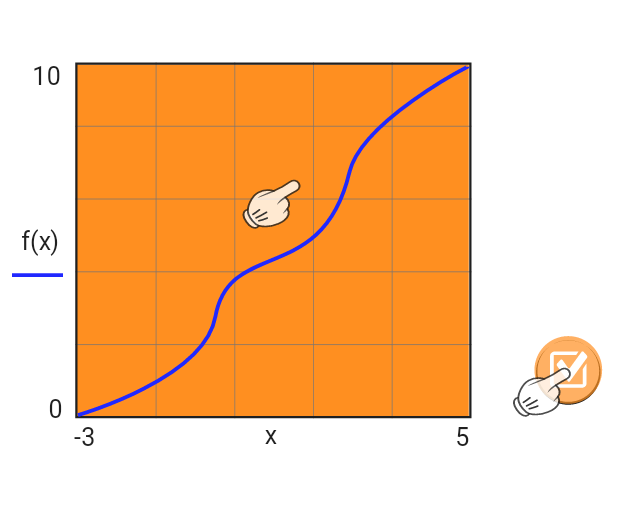
\includegraphics[resolution=320]{graphics/function_plot_fig3.png} \end{tabular}\end{center}
\begin{center}\begin{tabular}{c} 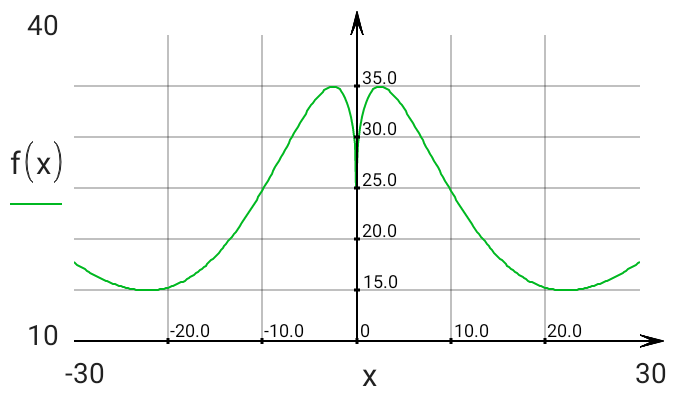
\includegraphics[resolution=320]{graphics/function_plot_fig4.png} \end{tabular}\end{center}

By long click on the middle of plot
area, the context menu and the
floating button ''Object properties''
will appear.
\begin{center}\begin{tabular}{c} 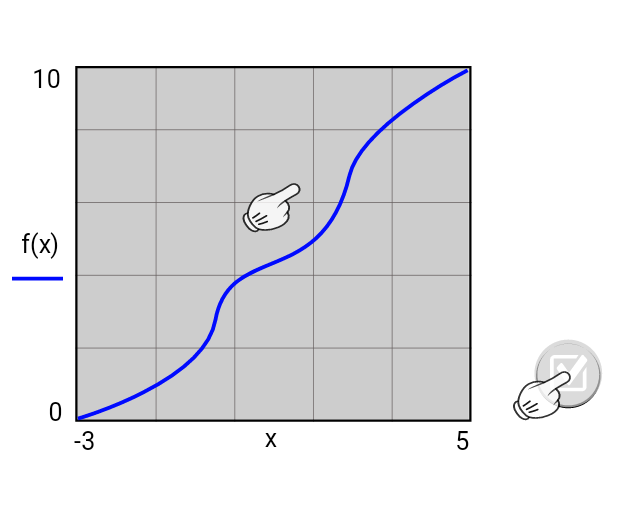
\includegraphics[resolution=320]{graphics/function_plot_fig5.png} \end{tabular}\end{center}

If you press this floating button, the
''Plot Settings'' dialog will be
displayed. Here, you can change size
and style of the plot area. For
example, the crossed graph looks like
this:
\begin{center}\begin{tabular}{c} 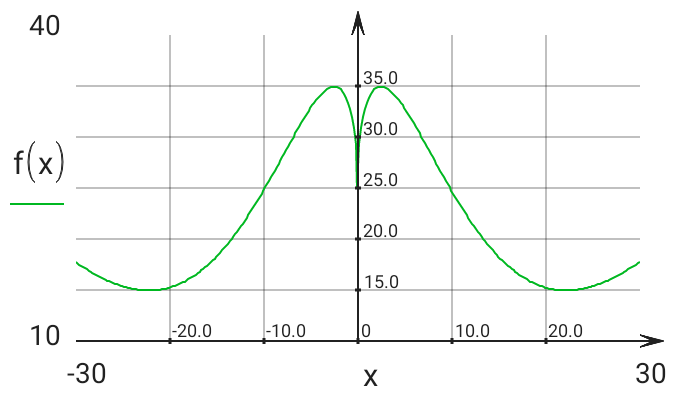
\includegraphics[resolution=320]{graphics/function_plot_fig6.png} \end{tabular}\end{center}

You can also change the plot line
color, width and style in the ''Line
Settings'' dialog. It appears by long
click on the line marker below the
function name on the left of plot
area:
\begin{center}\begin{tabular}{c} 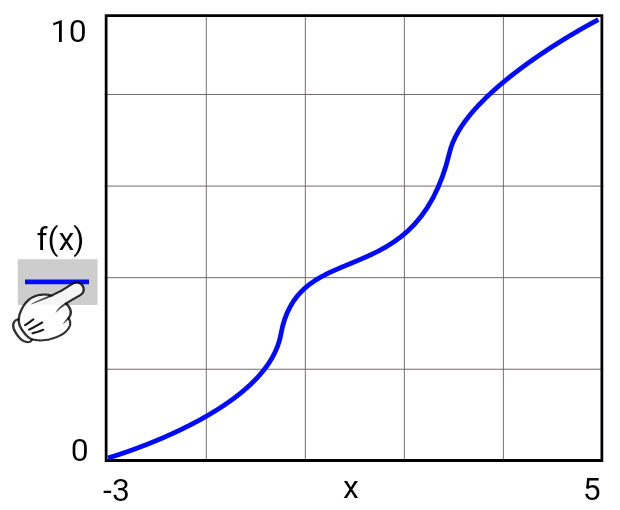
\includegraphics[resolution=320]{graphics/function_plot_fig7.png} \end{tabular}\end{center}

For example, we can use dotted lines:
\begin{center}\begin{tabular}{c} 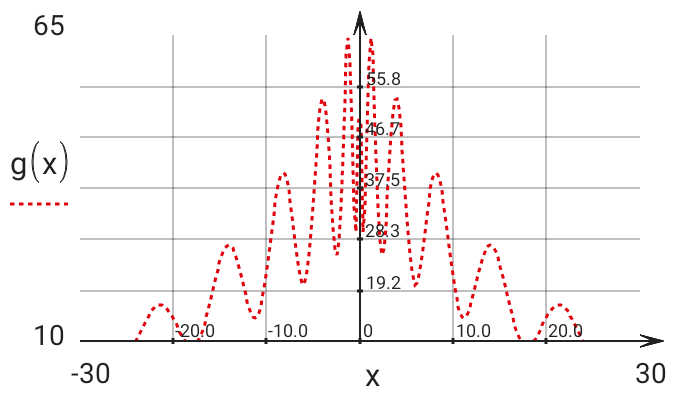
\includegraphics[resolution=320]{graphics/function_plot_fig8.png} \end{tabular}\end{center}

The number of axis labels and grid line
color can be changed in the ''Grid
Settings'' dialog. It appears by long
click on the free space between the x
minimum value (-30) and the argument
(x) symbol or between the x symbol and
the x maximum value (30) below the
plot area:
\begin{center}\begin{tabular}{c} 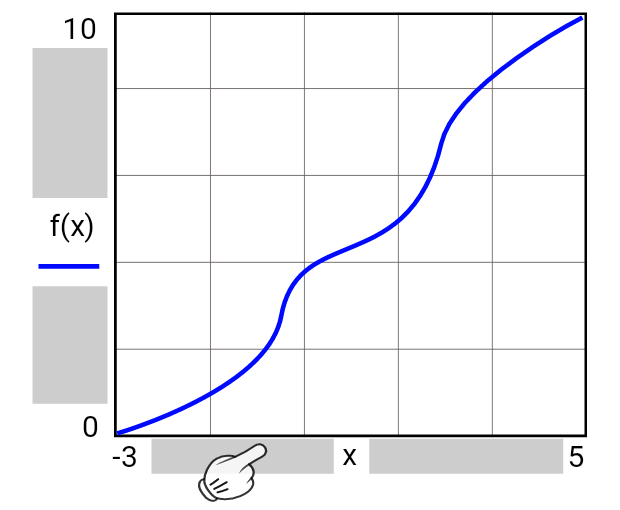
\includegraphics[resolution=320]{graphics/function_plot_fig9.png} \end{tabular}\end{center}
\begin{center}\begin{tabular}{c} 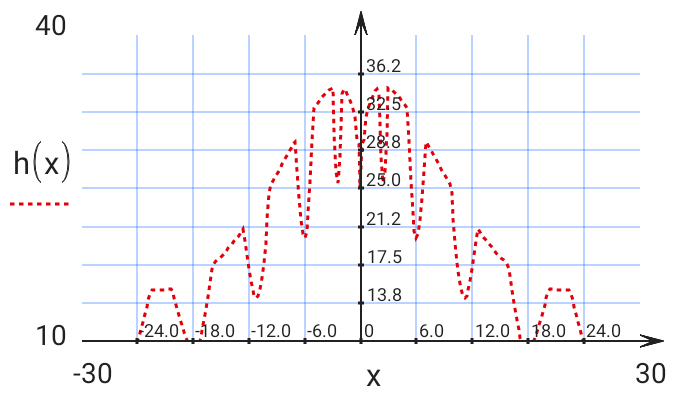
\includegraphics[resolution=320]{graphics/function_plot_fig10.png} \end{tabular}\end{center}

To hide grid completely just set the
number of grid lines to zero for both
vertical and horizontal axes.